% how to make a figure with text anotations

\documentclass{standalone}
\usepackage{xcolor}
\usepackage{graphicx}

\begin{document}

\setlength{\unitlength}{1mm}
\begin{picture}(90,32)
\put(0,1){
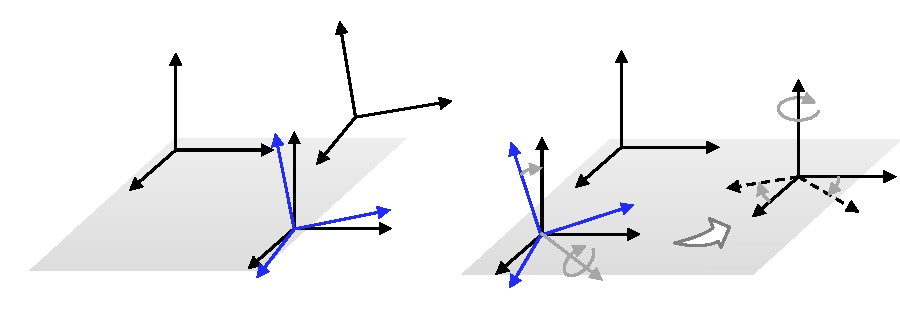
\includegraphics[width=0.725\linewidth]{frames-bare.pdf}
}
\put(25,   1){\small (a)}
\put(65,   1){\small (b)}
\put(7,  7.5){\small SE(2)}
\put(11,  19){\small $\{W\}$}
\put(55,  21){\small $\{W\}$}
\put(22,  10){\small $\{B\}$}
\put(46,   9){\small $\{B\}$}
\put(28,   6){\small \textcolor{blue}{$\{S\}$}}
\put(51,   3){\small \textcolor{blue}{$\{S\}$}}
\put(60,   5){\small \textcolor{gray}{$\bf a$}}
\put(36,  24){\small $\{C\}$}
\put(80,  18){\small $\{B\}$}
\put(59,  14){\small $x$}
\put(67,  17){\small $y$}
\put(59,  26){\small $z$}
\end{picture}


\end{document}